Das Erfassen von Supplierungen kann im Menü \enquote{Data Input} gestartet werden (siehe \autoref{fig:instr_substitudes_dataInput}). Es wird die Eingabemaske für die Abteilung des Users geöffnet (siehe \autoref{fig:instr_substitudes_subNoFree}). Der Super-User muss zuerst die zu bearbeitende Abteilung auswählen (siehe \autoref{fig:instr_substitudes_subSuUs}).
\begin{figure}[H]
\centering
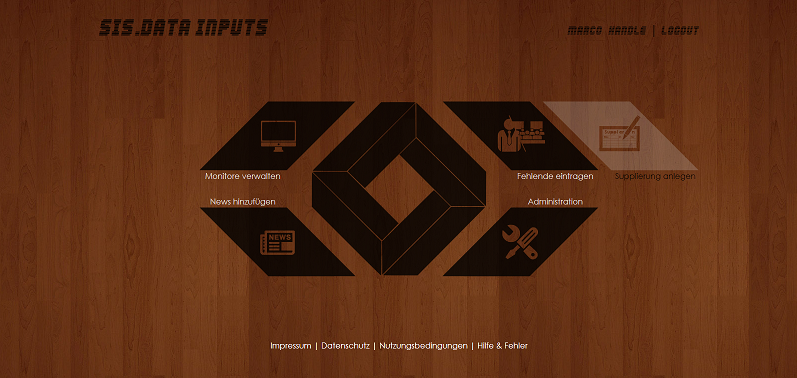
\includegraphics[keepaspectratio=true, width=14cm]{images/screenshots/data-inputs_substitudes.png}
\caption{Data-Input-Menü}
\label{fig:instr_substitudes_dataInput}
\end{figure}
\begin{figure}[H]
\centering
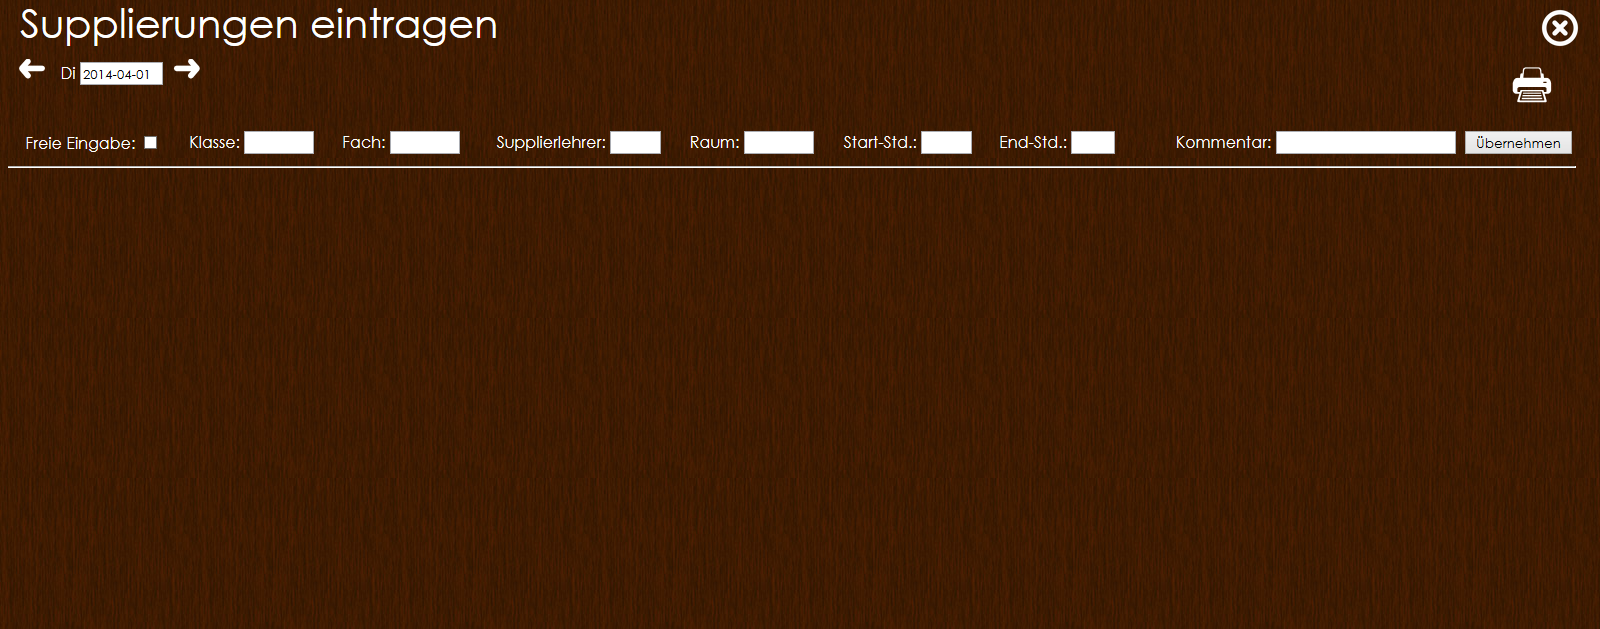
\includegraphics[keepaspectratio=true, width=14cm]{images/screenshots/substitudes_nofree.png}
\caption{Eingabemaske normal}
\label{fig:instr_substitudes_subNoFree}
\end{figure}
\begin{figure}[H]
\centering
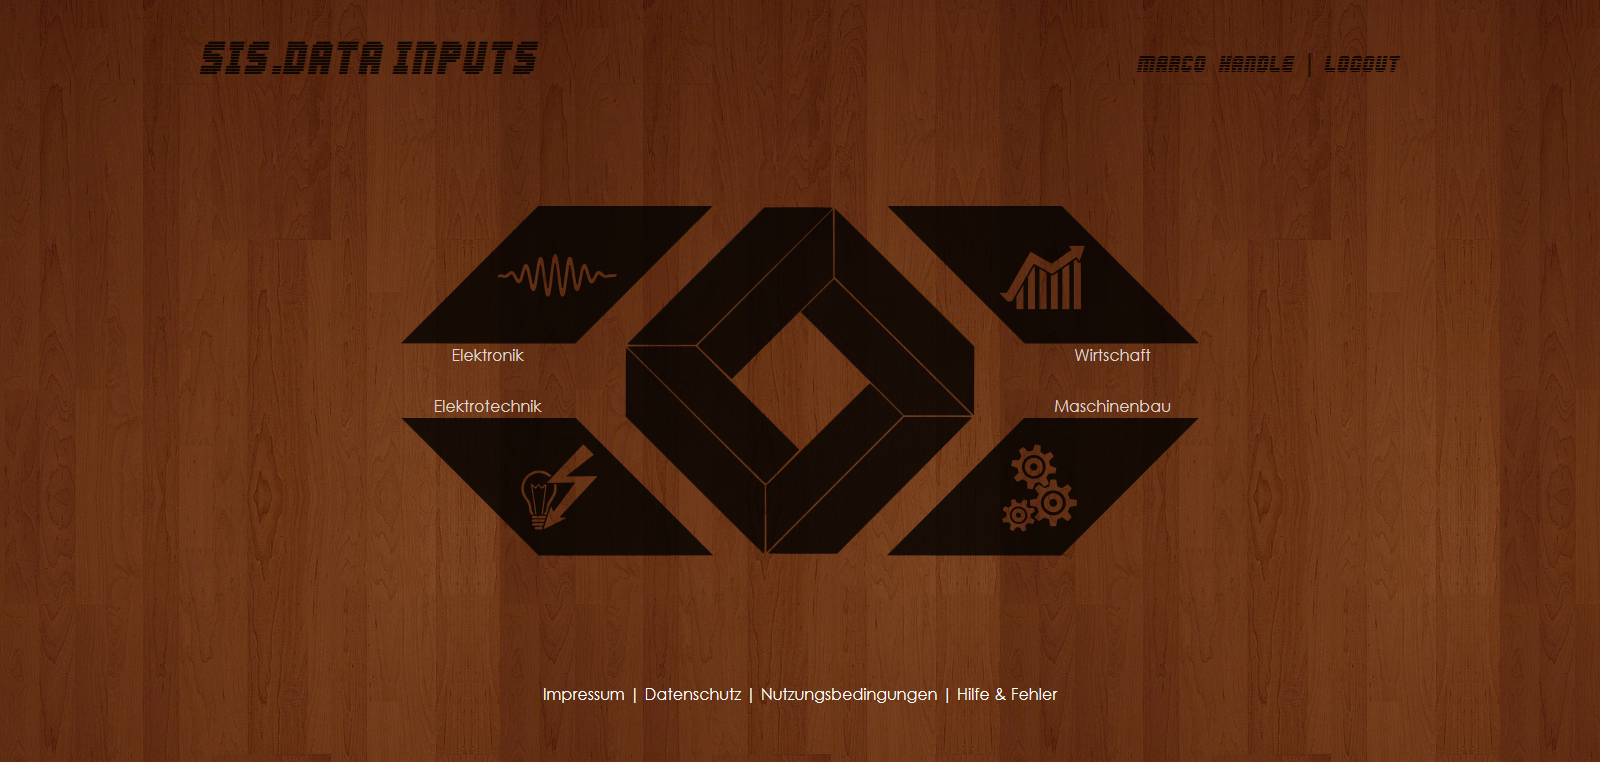
\includegraphics[keepaspectratio=true, width=14cm]{images/screenshots/substitudes_sections.png}
\caption{Super User Auswahl}
\label{fig:instr_substitudes_subSuUs}
\end{figure}
Es gibt 4 grundlegende Eingabevarianten:
\begin{itemize}
	\item Normale Eingabe\\
		siehe \autoref{sec:instr_admin_sub_noFree}
	\item Freie Eingabe\\
		siehe \autoref{sec:instr_admin_sub_Free}
		\begin{itemize}
			\item Stunde verschieben\\
				siehe \autoref{sec:instr_admin_sub_move}
			\item Stunde hinzufügen\\
				siehe \autoref{sec:instr_admin_sub_add}
			\item Stunde entfällt\\
				siehe \autoref{sec:instr_admin_sub_remove}
		\end{itemize}
\end{itemize}
\subsection{Normale Eingabe}\label{sec:instr_admin_sub_noFree}
Diese Eingabemethode (siehe \autoref{fig:instr_substitudes_subNoFree}) dient zur Erfassung von Supplierstunden von Klassen, deren Lehrer vorher als fehlend definiert wurde. Fehlen mehrere Lehrer in einer Klasse zur selben Zeit (Labor, FTKL, ...) ist die Freie Eingabe (siehe \autoref{sec:instr_admin_sub_Free}) zu verwenden.
\begin{table}[H]
\centering
\begin{tabular}{p{3 cm}p{6 cm}p{5 cm}}
   \toprule
   \textbf{Eingabefeld} & \textbf{Typ} & \textbf{Wertebereich} \\
   \midrule
          Freie Eingabe & Checkbox \newline nicht genutzt & \\
          \hline
          \textbf{Klasse} & Listenfeld - Pflichtfeld & Abteilungs-abhängig \\
          \hline
          Fach & Listenfeld - optional & \\
          \hline
          \textbf{Supplierlehrer} & Listenfeld - Pflichtfeld & \\
          \hline
          Raum & Listenfeld - optional & \\
          \hline
          \textbf{Start-Std.} & Erste Schulstunde der Supplierung  -Pflichtfeld & 1-16 \\
		  \hline
          \textbf{End-Std.} & Letzte Schulstunde der Supplierung  -Pflichtfeld & 1-16 \newline größer oder gleich Start-Std.\\
          \hline
          Kommentar & Textfeld - optional & \\
   \bottomrule
\end{tabular}
\caption{Eingabefelder normale Eingabe}
\end{table}
Mit der Schaltfläche Übernehmen wird eine Plausibilitätsüberprüfung vorgenommen und bei fehlerfreier Eingabe die Supplierstunde übernommen. Bei einer Fehleingabe wird der Fehler angezeigt und muss korrigiert werden. Nach der korrekten Übernahme wird die Checkbox Löschen in der erfassten Eingabezeile eingeblendet.
\subsection{Freie Eingabe} \label{sec:instr_admin_sub_Free}
Mit der Freien Eingabe können auch Supplierstunden erfasst werden, wenn der ursprüngliche Lehrer nicht fehlt. Um diese Methode auszuwählen muss in der Eingabemaske die Checkbox Freie Eingabe gesetzt werden. Es erscheinen zusätzliche Eingabefelder und drei Radio-Buttons zur Auswahl der Eingabemethode.\\
Standardmäßig ist der Radio-Button Verschiebung ausgewählt. Bei einer anderen Wahl ändern sich die Eingabefelder.
\subsubsection{Verschieben von Schulstunden} \label{sec:instr_admin_sub_move}
Diese Eingabemethode dient dazu:
\begin{itemize}
	\item Schulstunden einer Klasse innerhalb eines Tages zu verschieben
	\item Supplierstunden von 2 oder mehreren fehlenden Lehrern zu erfassen (Vertretung)
	\item Mehrstündige Fächer zu kürzen
\end{itemize}
Zur normalen Eingabemaske sind 3 zusätzliche Felder zu erfassen (siehe \autoref{fig:instr_substitudes_subMove}).
\begin{table}[H]
\centering
\begin{tabular}{p{3 cm}p{6 cm}p{5 cm}}
   \toprule
   \textbf{Eingabefeld} & \textbf{Typ} & \textbf{Wertebereich} \\
   \midrule
          \textbf{Freie Eingabe} & Checkbox \newline gesetzt & \\
          \hline
          \textbf{Klasse} & Listenfeld - Pflichtfeld & Abteilungs-abhängig \\
          \hline
          Fach & Listenfeld - optional & \\
          \hline
          Supplierlehrer & Listenfeld - Optional & \\
          \hline
          Raum & Listenfeld - optional & \\
          \hline
          \textbf{Start-Std.} & Erste Schulstunde der Supplierung  -Pflichtfeld & 1-16 \\
		  \hline
          \textbf{End-Std.} & Letzte Schulstunde der Supplierung  -Pflichtfeld & 1-16 \newline größer oder gleich Start-Std.\\
          \hline
          Kommentar & Wird automatisch mit \enquote{Verschiebung von} befüllt & \\
          \hline
          \textbf{Radio-Button} & \textbf{Verschiebung} - gesetzt\newline Hinzufügen - nicht gesetzt \newline Entfällt - nicht gesetzt & \\
          \hline
          \textbf{Urs. Start-Std.} & Erste ursprüngliche Schulstunde der Supplierung  -Pflichtfeld & 1-16 \\
          \hline
          \textbf{Urs. End-Std.} & Letzte ursprüngliche Schulstunde der Supplierung  -Pflichtfeld & 1-16 \newline größer oder gleich Urs. Start-Std.\\
          \hline
          Urs. Lehrer & Listenfeld - Optional \newline ursprünglicher Lehrer der Supplierung\\
   \bottomrule
\end{tabular}
\caption{Eingabefelder Verschiebung}
\end{table}
Einige der optionalen Informationen werden automatisch mit den Daten der ursprünglichen Stunde befüllt. Der ursprüngliche Lehrer kann/muss aber nicht angegeben werden. Wird er nicht angegeben, werden alle Stunden, die die Klasse zu der angegebenen Zeit hat, verschoben. Wenn die Klasse geteilt ist, alle Teilungen auch.\\
Mit der Schaltfläche Übernehmen wird eine Plausibilitätsüberprüfung durchgeführt und bei fehlerfreier Eingabe übernommen. Bei einer Fehleingabe wird der Fehler angezeigt und muss korrigiert werden. Nach der korrekten Übernahme wird die Checkbox Löschen in der erfassten Eingabezeile eingeblendet.
\begin{figure}[H]
\centering
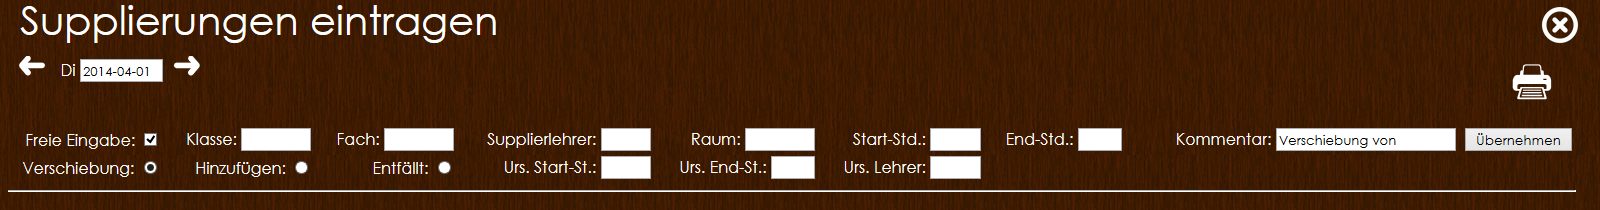
\includegraphics[keepaspectratio=true, width=14cm]{images/screenshots/substitudes_move.png}
\caption{Eingabemaske Verschiebung}
\label{fig:instr_substitudes_subMove}
\end{figure}
\subsubsection{Hinzufügen}\label{sec:instr_admin_sub_add}
Diese Eingabemethode dient dazu, zusätzliche Schulstunden an einem Tag einzufügen. Der neue Eintrag überschreibt den ursprünglichen Stundenplan der Klasse für diesen Tag.\\
Die Eingabemaske entspricht jener der Normalen Eingabe und enthält zusätzlich die Radio-Buttons (siehe \autoref{fig:instr_substitudes_subAdd}).
\begin{table}[H]
\centering
\begin{tabular}{p{3 cm}p{6 cm}p{5 cm}}
   \toprule
   \textbf{Eingabefeld} & \textbf{Typ} & \textbf{Wertebereich} \\
   \midrule
          \textbf{Freie Eingabe} & Checkbox \newline gesetzt & \\
          \hline
          \textbf{Klasse} & Listenfeld - Pflichtfeld & Abteilungs-abhängig \\
          \hline
          \textbf{Fach} & Listenfeld - optional & \\
          \hline
          \textbf{Supplierlehrer} & Listenfeld - Pflichtfeld & \\
          \hline
          Raum & Listenfeld - optional & \\
          \hline
          \textbf{Start-Std.} & Erste Schulstunde  -Pflichtfeld & 1-16 \\
		  \hline
          \textbf{End-Std.} & Letzte Schulstunde -Pflichtfeld & 1-16 \newline größer oder gleich Start-Std.\\
          \hline
          Kommentar & Textfeld - optional & \\
          \hline
          \textbf{Radio-Button} & Verschiebung - nicht gesetzt\newline 
          \textbf{Hinzufügen} - gesetzt \newline Entfällt - nicht gesetzt & \\
   \bottomrule
\end{tabular}
\caption{Eingabefelder Hinzufügen}
\end{table}
Mit der Schaltfläche Übernehmen wird eine Plausibilitätsüberprüfung durchgeführt und bei fehlerfreier Eingabe übernommen. Bei einer Fehleingabe wird der Fehler angezeigt und muss korrigiert werden. Nach der korrekten Übernahme wird die Checkbox Löschen in der erfassten Eingabezeile eingeblendet.
\begin{figure}[H]
\centering
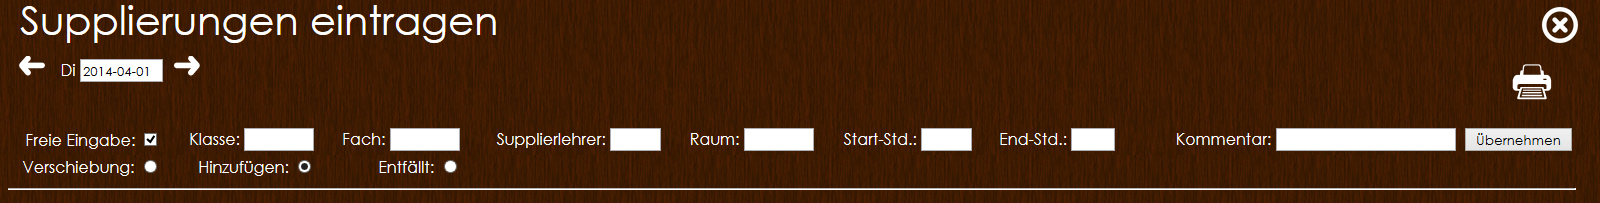
\includegraphics[keepaspectratio=true, width=14cm]{images/screenshots/substitudes_add.png}
\caption{Eingabemaske Hinzufügen}
\label{fig:instr_substitudes_subAdd}
\end{figure}
\subsubsection{Entfallen}\label{sec:instr_admin_sub_remove}
Entfällt eine Schulstunden ersatzlos, ist der Radio-Button Entfällt zu setzen. Die angegebene Stunde wird im Stundenplan der Schüler und Lehrer gelöscht.\\
Die Eingabemaske wird auf die unbedingt notwendigen Felder reduziert (siehe \autoref{fig:instr_substitudes_subRemove}).
\begin{table}[H]
\centering
\begin{tabular}{p{3 cm}p{6 cm}p{5 cm}}
   \toprule
   \textbf{Eingabefeld} & \textbf{Typ} & \textbf{Wertebereich} \\
   \midrule
          \textbf{Freie Eingabe} & Checkbox \newline gesetzt & \\
          \hline
          \textbf{Klasse} & Listenfeld - Pflichtfeld & Abteilungs-abhängig \\
          \hline
          Kommentar & Wird automatisch mit \enquote{entfällt} befüllt & \\
          \hline
          \textbf{Radio-Button} & Verschiebung - nicht gesetzt\newline Hinzufügen - nicht gesetzt \newline \textbf{Entfällt} - gesetzt & \\
          \hline
          \textbf{Urs. Start-Std.} & Erste ursprüngliche Schulstunde die Entfällt  -Pflichtfeld & 1-16 \\
          \hline
          \textbf{Urs. End-Std.} & Letzte ursprüngliche Schulstunde die Entfällt  -Pflichtfeld & 1-16 \newline größer oder gleich Urs. Start-Std.\\
          \hline
          \textbf{Urs. Lehrer} & Listenfeld - Pflichtfeld \newline ursprünglicher Lehrer der entfallenen Schulstunde\\
   \bottomrule
\end{tabular}
\caption{Eingabefelder Entfällt}
\end{table}
Mit der Schaltfläche Übernehmen wird eine Plausibilitätsüberprüfung durchgeführt und bei fehlerfreier Eingabe übernommen. Bei einer Fehleingabe wird der Fehler angezeigt und muss korrigiert werden. Nach der korrekten Übernahme wird die Checkbox Löschen in der erfassten Eingabezeile eingeblendet.
\begin{figure}[H]
\centering
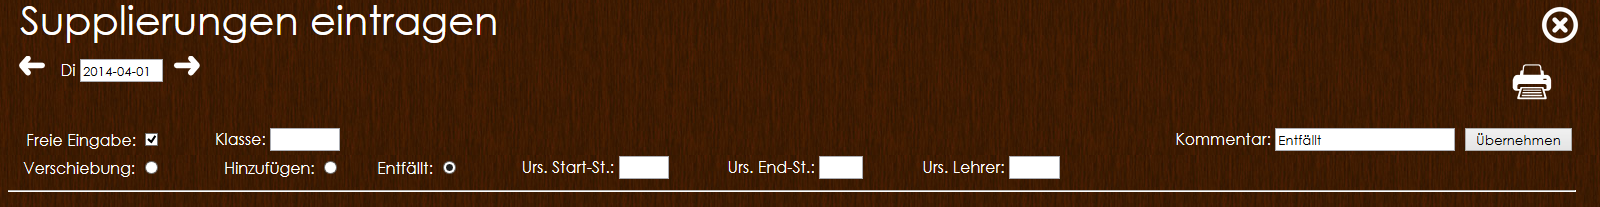
\includegraphics[keepaspectratio=true, width=14cm]{images/screenshots/substitudes_remove.png}
\caption{Eingabemaske Entfallen}
\label{fig:instr_substitudes_subRemove}
\end{figure}
\subsection{Fehler}
Wird in einem Eingabefeld ein Wert eingegeben, der nicht in der angezeigten Liste vorkommt oder nicht im Wertebereich liegt, wird ein Fehler zurückgegeben. In einem Pop-Up wird der Name des fehlerhaften Eingabefeldes angezeigt. Das Pop-Up ist mit der Schaltfläche Ok zu bestätigen. Anschließend muss die Eingabe erneut erfolgen.\\
Eine weitere Fehlerquelle kann darin liegen, dass bei der normalen Eingabe (siehe \autoref{sec:instr_admin_sub_noFree}) zur Erfassung einer Supplierung ein ursprünglicher Lehrer gewählt wird, der nicht als fehlend erfasst wurde oder wenn die ursprüngliche Stunde nicht gefunden wird. Diese Fehler werden unter der Seitenüberschrift angezeigt und die Trennlinie unter der Eingabezeile wird rot (siehe \autoref{fig:instr_substitudes_fail}).
\begin{figure}[H]
\centering
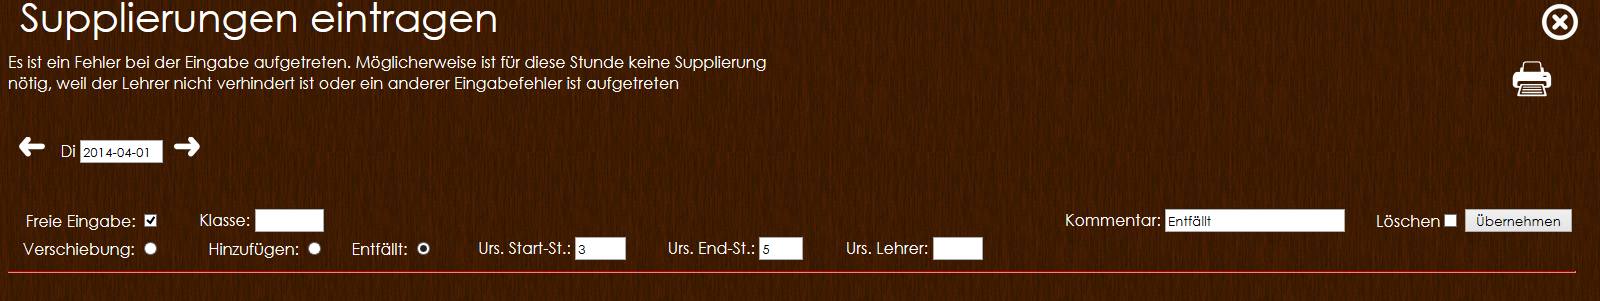
\includegraphics[keepaspectratio=true, width=14cm]{images/screenshots/substitudes_fail.png}
\caption{Fehleingabe}
\label{fig:instr_substitudes_fail}
\end{figure}
\subsection{Einträge ändern}
Bestehende Einträge können durch überschreiben geändert werden. Die Änderungen werden nach dem Drücken auf die Schaltfläche Übernehmen der Eingabezeile übernommen, sofern kein Fehler auftritt. Bei einer Fehlermeldung ist die Eingabe entsprechend zu korrigieren.
\subsection{Löschen}
Das Löschen eines Eintrages erfolgt über die Checkbox Löschen der entsprechenden Eingabezeile. Diese muss gesetzt und dann mit Übernehmen bestätigt werden. Es erfolgt keine weitere Sicherheitsabfrage und ist der Eintrag unwiderruflich gelöscht